Nowadays, the need for the visualization of software quality metrics has been rapidly increased. Software metrics help developers and companies to check and analyze information about the performance, quality of code and cost of software data. it helps to find out and fix errors in the early stages of development.

In this chapter will be described some tools for visualization of software quality metrics and tool for code analysis.

\section{Open Source tool "METRIX"}

This tool can compute different software quality metrics. METRIX is able to evaluate software written in C and ADA languages and many metrics can be considered for software evaluation (the different metrics will be described in detail in the next section~\cite{metrix}. 

Different diagrams enable the user to visualize numeric data. Graphics like line charts, scatter plots and histograms are common. 
There are two less-common classes of diagrams: 
\begin{itemize}
	\item The radar plots, also called Kiviat diagrams.
	\item The city map diagram, mostly used to represent the cartography of cities.
\end{itemize}
One specific feature of METRIX is to use those two types of visualization for constructing signature and cartography of source codes.
 
\textbf{Kiviat diagrams}
The Kiviat diagram visualizes information through polar coordinates. The distance between the point and the origin is associated to the value user want to represent, while the angle between two points is constant, this constant is uninformative and calculated to uniformly distribute the different points. Moreover, all metric points are linked together, making a plain polygon, which shapes the specificity of the data that the user wants to represent. Of course, this diagram is not adequate to represent only one or two metrics, it requires at least three values to be pertinent. Values may be of the same metrics, representing the metric measured on different parts of the source code. Values may be of very different metrics, computed  with heterogeneous units. That enables the user to merge multivariate data on the same diagram. On Kiviat diagrams, values must be strictly positive. 

In figure\ref{fig:metrix} shows an example of two Kiviat diagrams. These diagrams represent coding different metric values for two functions. 

\begin{figure}[h]
	\centering
	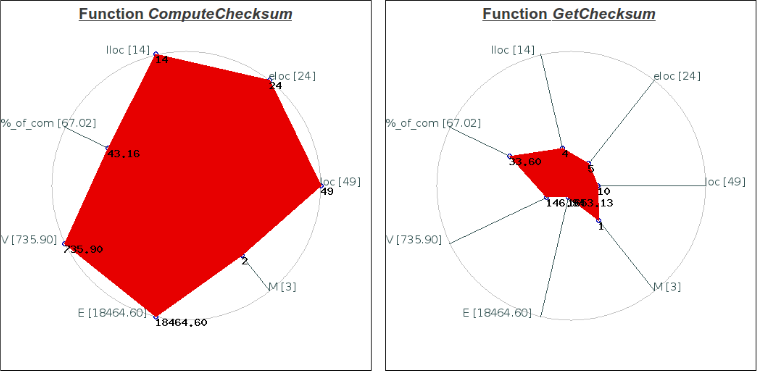
\includegraphics[height=70mm]{figures/metrix.png}
	\caption{An example of Kiviat diagrams.}
	\label{fig:metrix}
\end{figure}

\textbf{City map diagrams}
This diagram is mainly used in urbanism, to represent cities and their buildings in three dimensions. As a software project  can contain a very large number of source files, code functions  and code variables, but this visualization diagram adequately suits for complexity visualization issue. 

The treemap diagram is used in computing to represent in two dimensions source code metrics with rectangles. Some authors used variants of this class of visualization diagrams to represent  values with esthetic considerations. City map diagrams are indeed multi-parameters diagrams: each “building” is associated with an n-tuple of numeric values.  

This tool also has a graphical user interface with a single Window containing three tabs.

The first tab called “Calc” and enables the user to indicate the source file(s) to evaluate and to parameterize the metrics to compute. It avoids using hand-start scripts with a prompt, but the open source aspect of the tool allows advanced users to reuse the measuring scripts manually and/or to integrate them into other software.

The second tab called “Csv” presents the numeric values as a list, with a tab per function and per file. The user may export these values to a spreadsheet application, in order to represent  the values with common visualization graphs, like scatter plots, line plots, etc.

The third tab called “Plots” and provides a way to visualize the city map diagrams for the source code, the signatures of functions and the comparisons between functions through radar/Kiviat plots. This tab enables the user to change the default behavior of the tool, for example, to modify the ceiling and floor to insert color into the data, to adapt the placement of the buildings in the city map, etc. 

This tool may generate a report in the form of a LaTeX file, so the user can use it to produce a PDF file. This report summarizes all the values measured on the project. Each function and each file make a section of this report. In each section, numerical values are coupled with the signature of the function (as a Kiviat diagram). Each file produces three views of the associated city map diagram, as well as different Kiviat diagrams for the different metrics measured on the functions of the file. 

\section{Sextant}

Sextant is a Java source-code analysis tool under development at the University of Nebraska at Omaha (UNO)~\cite{sextant}. This software is a complex extension of the TL system (a general-purpose program transformation system) created particularly for the Java programming language domain.

The main design goal of Sextant is providing a tool facilitating specification and visualization of custom analysis rules, which can be domain-specific or moreover application specific analysis rules.

Analysis rules of Sextant are based on information fetched from different software models. There are two main models of central importance. The first model is a syntactic model. It is the source code parse tree. Parse trees conform to compilation units which represented by Java files and are generated with use of GLR parser technology provided by the TL system. Parse trees are well-fitted for analyzing and manipulating through standard primitives provided by program transformation systems, for example, by matching and generic traversal.

The second model is a compound attributed graph (CAG). It is a semantic model which captures subtype, structural, and reference dependencies among the constructors, methods, fields, packages and types. The CAG also links an attribute list with every node and edge.

CAG information is accessible to Sextant’s transformation-based analysis rules via two mechanisms. The first mechanism is a positional system which organizes a relation between contexts within the CAG and corresponding parse (sub)trees. This relation makes possible correctly resolving references to constructors, methods, types, fields, and local variables, during the process of generic traversals which are the key enabling mechanism in program transformation systems.

The second mechanism is a library of semantic queries. These queries can be accessed even in the middle of transformation course. Functionality which provided by this library contains things like:
\begin{itemize}
	\item Reference resolving.
	\item Reference type determining.
	\item Determining declaration shadowing or overriding.
	\item Determining whether one type is a subtype of another.
\end{itemize}
 
Sextant stores table and set types for information collecting with relation to analysis rules. These constructs can be used for storing information related to a custom metrics wide variety.

Sextant is open-ended with respect to the definition of metrics – any source-code analysis rule can be interpreted as a metric, be they PMD-style rules focusing on violations of coding conventions or rules such as those specified by FindBugs that are more semantic in nature\cite{sextant}.

Sextant can do software models generation. These models can be visualized using other tools such as GraphViz, Cytoscape and TreeMap. Sextant can produce the CAG of the code base in a JavaScript object notation format (JSON). This JSON file can be loaded into Cytoscape, an open source platform which provides extensive and sophisticated capabilities for large complex networks visualization, for example, graph structures. The same way, metrics derived from sets and tables can be produced in CSV format and viewed with use of TreeMap. Parse trees can be output as dot-files and later viewed with use of GraphViz.

The view in Figure\ref{fig:1} shows an example of represents a coloring of dependencies on the unsupported features. Nodes colored orange have indirect dependencies on unsupported features while purple nodes have direct dependencies on unsupported features.

\begin{figure}[h]
	\centering
	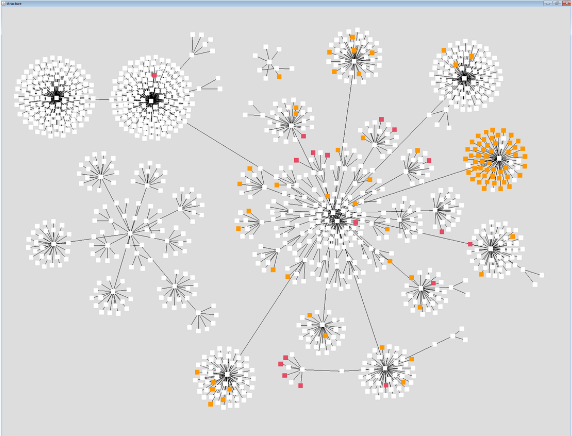
\includegraphics[height=70mm]{figures/1.png}
	\caption{An example of using Sextant tool.}
	\label{fig:1}
\end{figure}

\section{NDepend}

NDepend is a static analysis tool for .NET managed code. The tool supports a big number of code metrics, allowing to visualize dependencies using directed graphs and dependency matrix.  

NDepend computes a lot of size-related metrics: number of lines of code, number of assemblies, number of types, number of methods, etc. For measuring complexity, NDepend uses Cyclomatic Complexity. This metric measures the complexity of a type or a method by calculating the number of branching points in the code.
NDepend has two metrics for cohesion. Relational Cohesion is an assembly level metric that measures the average number of internal relationships per type. Lack of Cohesion Of Methods (LCOM) measures the cohesiveness of a type. A type is maximally cohesive if all methods use all instance fields.

NDepend uses a visualization tool called a Treemap.
NDepend comes with a dashboard to quickly visualize all application metrics s shown in Figure\ref{fig:dash}. The dashboard is available both in the Visual Studio extension. For each metric, the dashboard shows the diff since baseline. It also shows if the metric value gets better (in green) or wort (in red). 

\begin{figure}[h]
	\centering
	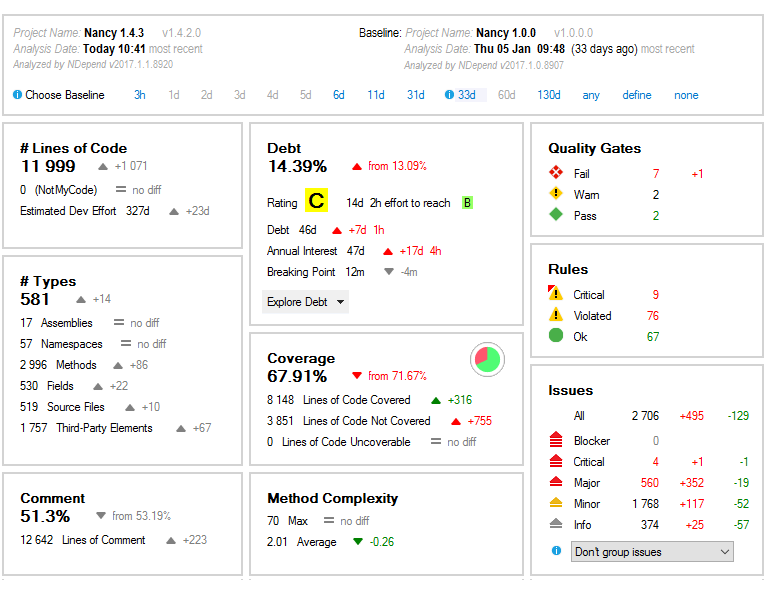
\includegraphics[height=70mm]{figures/dash.png}
	\caption{An example of using the dashboard.}
	\label{fig:dash}
\end{figure}

The Figure\ref{fig:tree} shows metric visualization using the colored treemap.

\begin{figure}[h]
	\centering
	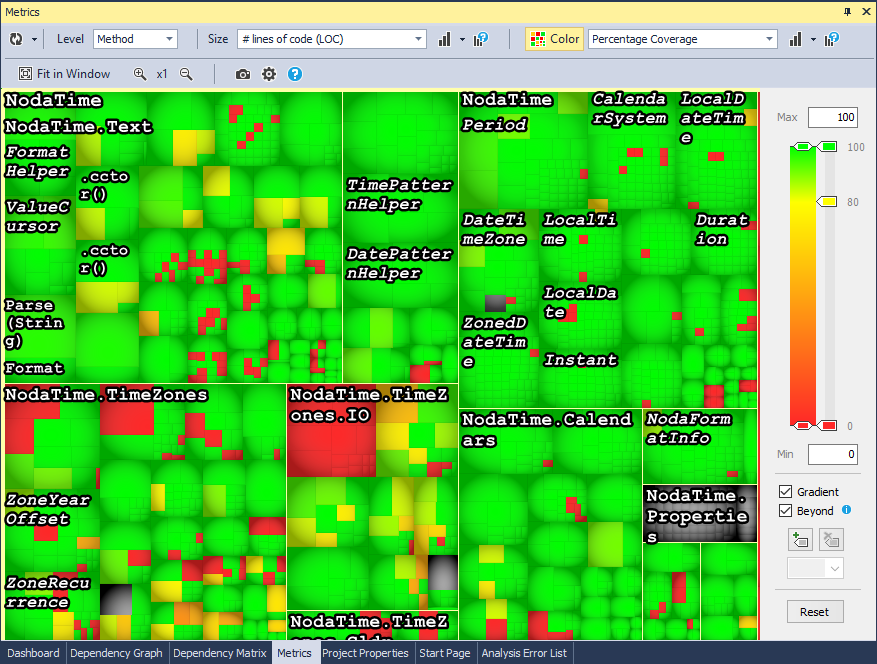
\includegraphics[height=70mm]{figures/tree.png}
	\caption{An example of using the colored treemap.}
	\label{fig:tree}
\end{figure}

The tree structure used in NDepend treemap is the usual code hierarchy: 

\begin{itemize}
	\item .NET assemblies contain namespaces.
	\item Namespaces contain types.
	\item Types contain methods and fields.
\end{itemize}

\section{PVS-Studio}

PVS-Studio is a tool for detecting bugs and security weaknesses in the source code of programs, written in C, C++, and C\#. It works in Windows, Linux, and macOS environment~\cite{pvs}.

This tool executes static code analysis and after that creates a report for helping developers to find and fix bugs. PVS-Studio has wide range check methods. It helps to find misprints and Copy-Paste errors. The main value of static analysis is in its regular use so that errors are identified and fixed at the earliest stages~\cite{pvs}. 

PVS-Studio runs from the command line. The analysis results can be saved as HTML with full source code navigation. It is possible to not include files from the analysis by name, folder or mask; to run the analysis on the files modified during the last N days. Error statistics can be viewed in Excel~\cite{pvs}. 

This tool has an online reference guide concerning all the diagnostics available in the program, on the website and documentation. 

PVS-Studio has an integration with open source platform SonarQube designed for continuous analysis and measurement of code quality.